\documentclass[11pt,letterpaper]{article}
\usepackage[T1]{fontenc}
\usepackage{lmodern,amsmath,amssymb,amsthm,graphicx,xcolor,booktabs,tabularx,array,enumitem}
\usepackage[margin=0.93in,top=0.80in,bottom=0.77in,headheight=15pt]{geometry}
\usepackage{microtype,fancyhdr,titlesec}
\usepackage[hidelinks]{hyperref}
\definecolor{ink}{HTML}{153D46}
\definecolor{accent}{HTML}{166568}
\hypersetup{colorlinks=true,linkcolor=accent,urlcolor=accent,citecolor=accent,
 pdftitle={Approximate Brouwer fixed points in intuitionistic primitive recursive arithmetic},
 pdfauthor={Research report prepared for Vladimir Reshetnikov}}
\pagestyle{fancy}\fancyhf{}
\lhead{\small\sffamily Approximate Brouwer fixed points}
\rhead{\small\sffamily Constructive arithmetic}
\cfoot{\small\sffamily\thepage}
\renewcommand{\headrulewidth}{0.25pt}
\titleformat{\section}{\large\bfseries\sffamily\color{ink}}{\thesection}{0.6em}{}
\titleformat{\subsection}{\normalsize\bfseries\sffamily\color{ink}}{\thesubsection}{0.6em}{}
\titlespacing*{\section}{0pt}{15pt}{6pt}
\titlespacing*{\subsection}{0pt}{10pt}{4pt}
\titlespacing*{\paragraph}{0pt}{7pt}{0.55em}
\setlength{\parindent}{1.1em}
\setlength{\parskip}{1.6pt plus 0.3pt}
\setlist{topsep=4pt,itemsep=3pt,parsep=0pt,leftmargin=*}
\setlength{\emergencystretch}{1em}
\raggedbottom
\newcommand{\N}{\mathbb N}\newcommand{\Q}{\mathbb Q}
\newcommand{\ipra}{\mathrm{iPRA}}\newcommand{\epsi}[1]{\varepsilon_{#1}}
\newcommand{\dist}{\operatorname{dist}_\infty}
\newcommand{\norm}[1]{\lVert #1\rVert_\infty}
\newcommand{\cube}{[0,1]^d}
\newcommand{\clip}{\operatorname{clip}}
\newcommand{\proofnamefont}[1]{\textsf{\textbf{#1}}}
\newtheoremstyle{claim}{6pt}{6pt}{\itshape}{}{\sffamily\bfseries\color{ink}}{.}{.5em}{}
\theoremstyle{claim}\newtheorem{theorem}{Theorem}\newtheorem{lemma}[theorem]{Lemma}
\newtheorem{corollary}[theorem]{Corollary}
\newcommand{\repo}[2]{\href{https://github.com/VladimirReshetnikov/ProveIt/blob/022dfb4c54c22782f927a903f25bcf6491b7eba2/Logic/PrimitiveRecursiveArithmetic/#1}{#2}}
\begin{document}
\thispagestyle{plain}
{\noindent\small\sffamily\bfseries\color{accent} CONSTRUCTIVE TOPOLOGY}\par\vspace{5pt}
{\noindent\fontsize{24}{28}\selectfont\sffamily\bfseries\color{ink} Approximate Brouwer fixed points}\par
{\noindent\large in intuitionistic primitive recursive arithmetic}\par\vspace{11pt}
\noindent
Given a requested error, we compute a rational point at which a uniformly
presented self-map moves the point by less than that error. The construction
works in every finite dimension on the simplex, the cube and the closed
Euclidean ball. Its arithmetic core is a parity calculation on finite tables.
The same grid point works at every sufficiently fine evaluation precision.
This is the approximate fixed-point property studied in constructive
analysis~\cite{kuhn,hendtlass}, applied to the classical domains
in~\cite{brouwer}.

\section{The theorem and its numerical content}
Write $\epsi m=2^{-m}$ and let
$\Delta^d=\{x\in\mathbb R^{d+1}:x_i\ge0,\ \sum_{i=0}^d x_i=1\}$.
We measure barycentric errors in the maximum norm.
A map is presented by an evaluator $A(x,s)$ with rational values in
$\Delta^d$ at rational points $x$, and a modulus $\mu$ with the following contract:
\begin{equation}
\label{eq:contract}
 s,t\ge m,\quad\norm{x-y}\le\epsi{\mu(m)}
 \quad\Longrightarrow\quad \norm{A(x,s)-A(y,t)}\le\epsi m .
\end{equation}
Both $A$ and $\mu$ are fixed primitive recursive (PR) terms, possibly with numerical
parameters such as the dimension or coefficients. Their inputs and outputs are
number codes. Section~\ref{sec:names} explains how to obtain this presentation
from the familiar approximation and continuity data.

\begin{theorem}[Uniform simplex approximation]\label{thm:main}
There is an explicit witness term $W$ for each pair of PR terms $A,\mu$.
From their contracts iPRA proves the following. For every $d,k\in\N$ put
\[
 m=k+2,\qquad N=2^{\max\{m,\mu(m)\}},\qquad x=W(d,k).
\]
Then $x$ is a barycentric grid point of denominator $N$, and for every $s\ge m$,
\begin{equation}\label{eq:main}
 \norm{x-A(x,s)}
 \ \le\ \frac{2d}{d+1}\bigl(N^{-1}+2^{-m}\bigr)
 \ \le\ \frac{d}{d+1}\,2^{-k}\ <\ 2^{-k}.
\end{equation}
The search visits at most $N^d$ cells. All calls that determine $x$ use
precision $m$. Dimension zero returns $(1)$.
\end{theorem}

In the metric completion, $f(x)=\lim_s A(x,s)$ satisfies the same first two bounds.
For any specified positive rational $\varepsilon$, choose $k$ with $2^{-k}\le\varepsilon$.
For $\varepsilon=a/b$ in positive integers, $k=b$ is already a PR bound for this choice.
The witness is an \emph{approximate fixed point in residual norm}. Even among
$1$-Lipschitz interval maps, a residual alone gives no uniform distance to an exact
fixed point. For example, $f(t)=(1-\lambda)t$, $0<\lambda\le1$, has unique fixed point zero
and residual $\lambda$ at $1$. Neither the statement nor its proof calls for a
convergent subsequence of the computed witnesses.

\section{What the map data represent}\label{sec:names}
In ordinary iPRA, as presented by ProveIt~\cite{ipra}, the only sort is
$\N$. It has symbols and defining equations for PR definitions, intuitionistic
first-order logic with equality, and induction for quantifier-free formulas.
For a numerical family $A(e,d,x,s),\mu(e,d,m)$, the assertion above is a
single arithmetic implication for all parameter values. Validity of the
presentation at those parameters is its antecedent. One can also use a new pair
of terms for each problem, giving a schema. The finite table theorem below
is a single numerical theorem even when every sample is supplied independently.

\paragraph{Evaluation and continuity.}
At $x=y$, \eqref{eq:contract} makes $A(x,s)$ a Cauchy name with a known
rate. At rational points of distance at most $2^{-\mu(m)}$, passing the
estimate to the limits gives the same $2^{-m}$ modulus. These limits uniquely
extend to the completion of the rational simplex. More explicitly, suppose
$u$ is given by rational points $x_l$ at distance at most $2^{-l}$ from $u$.
At output stage $m$, query $A(x_{L(m)},m)$ with
$L(m)=1+\max_{j\le m}\mu(j)$. For any $s,t\ge m$, the two input points
are at distance at most $2\cdot2^{-1-\mu(m)}$; \eqref{eq:contract} gives
output distance at most $2^{-m}$. The same comparison between two names for
$u$ proves independence of the name. Constant rational input names
recover the original values in the completion.

Conversely suppose a uniformly continuous $f$ has a supplied spatial modulus
$\nu$ and simplex-valued rational samples $B(x,s)$ within $2^{-s}$ of $f(x)$.
Take $A(x,s)=B(x,s+2)$ and $\mu(m)=\nu(m+1)$. The two sampling errors total
at most $2^{-m-1}$ and the spatial error is at most $2^{-m-1}$.
This proves~\eqref{eq:contract}. A supplied Lipschitz bound $L\le2^b$,
for instance, gives $\nu(m)=m+b$.

\paragraph{Making approximate coordinates simplex-valued.}
There is a rational correction that costs one bit in every dimension.
For an arbitrary $(d+1)$-tuple $b$ set
\[
 \tau(b)=\max_{\varnothing\ne S\subseteq\{0,\ldots,d\}}
       \frac{\sum_{i\in S} b_i-1}{|S|},\qquad
 \Pi_i(b)=\max\{0,b_i-\tau(b)\}.
\]
Every subset sum of $b_i-\tau(b)$ is at most $1$, and one is $1$.
The largest subset sum is the sum of the positive entries, hence
$\sum_i\Pi_i(b)=1$. If $b$ belongs to the simplex then $\tau(b)=0$
by using the full index set. Each displayed average varies by at most
$\norm{b-b'}$, so $\Pi$ is $2$-Lipschitz. Thus a rational sample within
$2^{-s-1}$ of a simplex point becomes a simplex-valued sample within
$2^{-s}$. The $2^{d+1}-1$ nonempty subsets are a PR enumeration.
The spatial modulus of a general pointwise continuous map remains
additional input.

\section{A finite Sperner lemma with its incidence proof}
\label{sec:finite-sperner}

Fix integers $N\geq 1$ and $d\geq 0$. Use cumulative coordinates for the
simplex grid,
\[
 G_d(N)=\{u\in\{0,\ldots,N\}^d: u_1\leq\cdots\leq u_d\}.
\]
Set $u_0=0$, $u_{d+1}=N$ and $a_i(u)=u_{i+1}-u_i$ for $0\leq i\leq d$.
The barycentric point represented by $u$ is $(a_0(u),\ldots,a_d(u))/N$.
The grid $G_0(N)$ consists of the empty tuple and its single gap is $N$.
A coloring is a table $c$ with values in $\{0,\ldots,d\}$ at grid points.
Its boundary condition is
\[
                       a_{c(u)}(u)>0\qquad(u\in G_d(N)).
\]

\paragraph{The cells.}
For $d>0$, take a sorted base $b\in\{0,\ldots,N-1\}^d$ and a permutation
$p_1,\ldots,p_d$ of $1,\ldots,d$. Its vertices are
\[
        v^0=b,\qquad v^s=b+\sum_{t=1}^s e_{p_t}
                     \quad(1\leq s\leq d).
\]
Keep this cell when all its vertices are sorted. Equivalently, within
each block of equal entries of $b$, the coordinates must be incremented
in decreasing index order. Indeed, incrementing the left of two equal
neighbors first violates their order. Two neighbors starting at distinct
integers stay ordered after either one is incremented once.
For $d=0$ use the single one-vertex cell. For any $s\leq t$ the
coordinates of $v^t-v^s$ belong to $\{0,1\}$. Extending this difference
by zero at the two endpoints shows
\begin{equation}\label{eq:sperner-gap-mesh}
              |a_i(v^t)-a_i(v^s)|\leq 1\qquad(0\leq i\leq d).
\end{equation}

The cells admit an enumeration with exactly $N^d$ entries. For a word
$w=(w_1,\ldots,w_d)\in\{0,\ldots,N-1\}^d$, sort it to obtain $b$.
Assign successive occurrences of each value in $w$ to the indices of its
block in $b$ from right to left. The index assigned to position $t$ is
$p_t$. The inverse reads $w_t=b_{p_t}$, because the validity criterion
uniquely fixes the order inside each block. This enumeration also works
for $N=1$ and for the empty word.

\paragraph{Finite Sperner lemma.}
For every coloring satisfying the boundary condition, the number of
cells with all $d+1$ colors is odd. The first such cell in word order can
therefore be found by scanning at most $N^d$ words.

\paragraph{Counting incidences.}
Suppose $d>0$. An incidence $(C,k)$ consists of a cell and the face
obtained by deleting its vertex $v^k$, $0\leq k\leq d$. Count it if the
remaining $d$ vertices carry precisely the colors $0,\ldots,d-1$.
A cell missing one of these colors contributes zero. If it contains
them all, its one remaining color occurrence either is $d$ or repeats
one of these colors. In the first case just the deletion of the
$d$-colored vertex counts. In the second case precisely the two
deletions of the repeated color count. Thus the parity of the incidence
count is the parity of the fully colored cell count.

Here is an explicit pairing on the incidences. The formulas preserve
the ordered list of retained vertices and hence preserve the counted
condition.
\begin{enumerate}
\item If $0<k<d$, interchange $p_k$ and $p_{k+1}$, using the same
deletion index $k$. Only the deleted vertex changes. If the interchange
is valid, applying it twice returns to the original cell. If it is
invalid, let $\ell=p_{k+1}$ and $y=v^{k-1}$. Increasing coordinate
$\ell$ first must violate $y_\ell\leq y_{\ell+1}$, so $\ell<d$ and
$y_\ell=y_{\ell+1}$. There is no possible overflow because $\ell$
has not yet been incremented. Since the vertex after both moves is
sorted, the other increment must be $p_k=\ell+1$. The two coordinates
are equal at every retained vertex, as neither has been incremented
before these moves and both have been incremented afterwards. All
retained vertices have $a_\ell=0$, so the missing color $\ell<d$
prevents this incidence from counting.
\item If $k=0$, let $j=p_1$. Use base $b+e_j$, order
$(p_2,\ldots,p_d,j)$, and delete the last vertex. Its first $d$ vertices
are the retained vertices of $C$. For $j<d$ the validity of the
original first move gives $b_j<b_{j+1}$, so the new last vertex is
sorted and within the coordinate bounds. For $j=d$, the additional
move is valid precisely when $b_d<N-1$. Thus the sole unpaired case
has $j=d$, $b_d=N-1$. Every retained vertex then has $u_d=N$.
\item If $k=d$, let $j=p_d$. Use base $b-e_j$, order
$(j,p_1,\ldots,p_{d-1})$, and delete the first vertex. This operation
inverts the preceding rotation whenever both are defined. If $j>1$,
the original penultimate vertex gives $b_{j-1}+1\leq b_j$, so the new
base is nonnegative and sorted. For $j=1$ the construction fails
precisely when $b_1=0$. In that case all retained vertices have
$u_1=0$, so none carries color zero and the incidence does not count.
\end{enumerate}

Each defined pairing exchanges distinct incidences. For the middle
deletion it changes a permutation, and at the ends it exchanges
deletion indices $0$ and $d$. Its counted pairs therefore contribute an
even number. The remaining counted incidences are exactly those of the
second case on $u_d=N$. Deleting the final coordinate of their retained
vertices gives cells in $G_{d-1}(N)$. Conversely, append $N-1$ to a
lower-dimensional base, prepend the step $d$ to its permutation, and
delete the initial vertex. These constructions are inverse. On the
top face the coloring $u'\mapsto c(u',N)$ satisfies the lower-dimensional
boundary condition because the last gap vanishes and the earlier gaps
are exactly the gaps of $u'$. Consequently the boundary contributes
exactly one incidence per fully colored lower-dimensional cell.
In dimension zero the unique vertex has color zero. This proves the
lemma by parity descent through the top faces.

\paragraph{The induction formula in iPRA.}
To justify that last descent uniformly in the dimension, fix the
ambient dimension $D$, $N$ and the entire finite color table $T$ as
parameters. For $r\leq D$ use its restriction
\[
 c_r(u_1,\ldots,u_r)=T(u_1,\ldots,u_r,
                           \underbrace{N,\ldots,N}_{D-r}).
\]
The positive-gap test on $T$ implies it for every restriction,
since all appended gaps beyond index $r$ vanish. Let $P(r)$ be the
number of fully colored $r$-cells modulo two computed by the word
enumeration on $c_r$. For a fixed parameter table the statement
$P(\min(r,D))=1$ is an equation of primitive recursive terms.
The dimension-zero computation starts its quantifier-free induction.
For $r<D$ the preceding incidence calculation gives
$P(r+1)=P(r)$, and for $r\geq D$ the capped index is constant.

All finite tests here may be implemented as Boolean folds. For example,
$T$ can use $(N+1)^D$ address slots in base $D+2$, with arbitrary
values at unused addresses and the support and range tests restricted
to sorted tuples. Word enumeration, bounded sorting, prefix sums,
permutation rotations and color counts are primitive recursive.
At dimension $r$ the incidence loop has exactly $(r+1)N^r$ entries.
For a formal counting justification, order the paired indices
numerically and group by the smaller index of each pair. Its fiber
consists of exactly its two members, since the pairing is an involution
without fixed points. Summing the indicator of the grouping relation
over the two finite indices in either order gives twice the number of
smaller members. The boundary bijection is checked by the same
double-sum argument with singleton fibers. Interchanging such finite
sums follows by quantifier-free induction on their bounds, with
bounded prefix sums as terms. All grid membership and incidence
checks have explicit finite enumerations. In particular, the induction
formula has no quantifier over possible color tables.



\section{Turning colors into a residual bound}\label{sec:residual}
Write $X(u)=a(u)/N$ for the point of the simplex encoded by a grid vertex.
Let $T$ be any table assigning a rational simplex point $q(u)$ to every
$u\in G_d(N)$. On this table there is no continuity assumption.

\begin{lemma}[Finite table certificate]\label{lem:finite}
A single PR procedure on $(d,N,T)$ returns a cell $C$ and the anchor
$x=X(v^0)$ with the following property. If $y\in\Delta^d\cap\Q^{d+1}$
and $\omega\ge0$ satisfy $\norm{y-q(v)}\le\omega$ at every vertex $v$
of $C$, then
\[
                     \norm{x-y}\le\frac{2d}{d+1}(N^{-1}+\omega).
\]
The checker for this implication needs only the $d+1$ rows of $C$.
\end{lemma}

\begin{proof}
At $v$, put $r_j=X_j(v)-q_j(v)$, and label $v$ by the least $i$ maximizing
$r_i$ among indices with $X_i(v)>0$. The support is nonempty. Outside it,
$r_j=-q_j(v)\le0$. The residuals on the support sum to
$\sum_{X_j(v)=0} q_j(v)\ge0$, so their maximum is nonnegative.
The chosen index is therefore a global maximizer. This tie rule matters
when $q(v)=X(v)$ on a face, since it still selects an index present on that face.

The support condition is exactly the hypothesis of the finite Sperner lemma.
Scan its words until all colors occur on a cell. Take its initial vertex as
anchor. For every color $i$ let $w_i$ be its vertex and set $R_j=x_j-y_j$.
By~\eqref{eq:sperner-gap-mesh} and the hypothesis on $y$, writing
$E=N^{-1}+\omega$, one has
\[
 |R_j-(X_j(w_i)-q_j(w_i))|\le E \qquad(0\le i,j\le d).
\]
At $w_i$ the largest residual is the $i$th. Comparing there and at the
anchor gives $R_j-R_i\le2E$ for every ordered pair. Since $\sum_i R_i=0$,
\[
 (d+1)R_j=\sum_i(R_j-R_i)\le 2dE,\qquad
 -(d+1)R_j=\sum_i(R_i-R_j)\le 2dE.
\]
In each sum the $i=j$ term vanishes. Division by the positive $d+1$
proves the estimate, including the singleton simplex.
\end{proof}

\begin{proof}[Proof of Theorem~\ref{thm:main}]
Use $q(v)=A(X(v),m)$ in Lemma~\ref{lem:finite}. For an arbitrary
$s\ge m$, take $y=A(x,s)$. Every $X(v)$ in the returned cell is within $1/N$
of $x$, which is at most $2^{-\mu(m)}$.
Contract~\eqref{eq:contract} gives $\omega=2^{-m}$. Substituting
$1/N\le2^{-m}$ and $m=k+2$ yields~\eqref{eq:main}. The scan
has finished before $s$ is chosen, so the same $x$ proves the entire tail
estimate.
\end{proof}

\subsection{A certificate that can be checked by hand}
Let $d=2$, $N=5$ and $f(x_0,x_1,x_2)=(x_1,x_2,x_0)$.
The cumulative vertices $(1,3),(2,3),(2,4)$ form a cell: increment the first
coordinate and then the second. At its anchor, $5x=(1,2,2)$ and
$5f(x)=(2,2,1)$. The figure gives all three residuals and the corresponding
labels. The oscillation of the three sample values is $1/5$, so the certified
bound is $8/15$. Direct evaluation gives the smaller residual $1/5$. The
exact fixed point $(1/3,1/3,1/3)$ lies off the grid.
\begin{center}
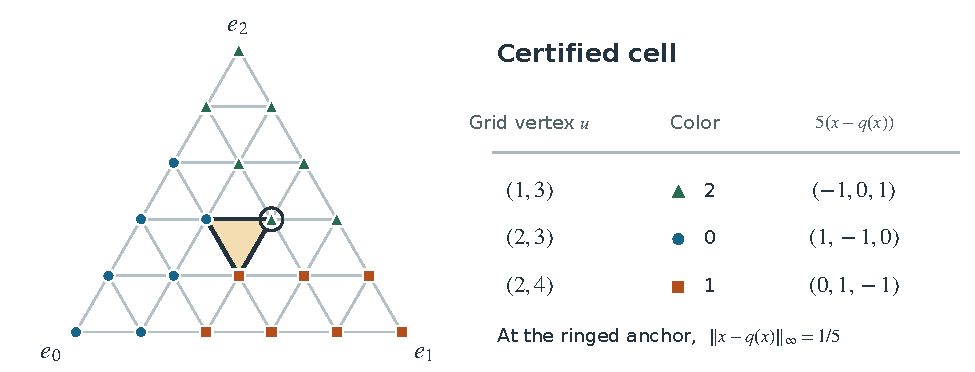
\includegraphics[width=0.91\linewidth]{figure.pdf}
\end{center}
A second example illustrates why the conclusion in Theorem~\ref{thm:main}
quantifies over $s$. Let $A(x,s)=(1-\alpha_s)f(x)+\alpha_s e_0$ with
$\alpha_s=2^{-s-2}$. Its mixed-stage variation is at most
$\norm{x-y}+|\alpha_s-\alpha_t|$, so $\mu(m)=m+1$ suffices.
For $k=1$ the program samples at stage $3$ on the $N=16$ grid.
It returns $(5/16,5/16,3/8)$, with certified residual at most $1/4$
at every stage $s\ge3$. The respective residuals at $s=3,4,8$
are $37/512,69/1024,1029/16384$. The theorem gives the remaining
infinitely many inequalities from the same finite certificate.

\section{The cube and the Euclidean ball}\label{sec:domains}
Throughout this section, a presentation on a domain uses its rational points
and contract~\eqref{eq:contract} in the maximum norm. An empty coordinate
tuple has norm zero. All retractions below map rational points to rational points.

\paragraph{How to transfer the witness.}
Let $D,X$ be two such domains and suppose $I:D\to X$, $P:X\to D$ are
rational PR functions with $PI=\mathrm{id}_D$. Suppose their maximum-norm
Lipschitz constants are at most $2^a$ and $2^b$, respectively. From a
presentation on $D$ form the $X$-presentation
\[
 H(u,s)= I(A(P(u),s+a)),\qquad \mu_H(m)=b+\mu(m+a).
\]
For $s,t\ge m$ the shifted evaluation stages are at least $m+a$.
The Lipschitz estimate for $P$ and the input radius
$2^{-b-\mu(m+a)}$ allow the contract for $A$ at level $m+a$.
Applying $I$ gives output distance at most $2^{-m}$.
If $u$ has residual at most $\delta$ for $H$ at stage $s$, then
$x=P(u)$ has residual at most $2^b\delta$ for $A$ at stage $s+a$. Apply $P$ to $u$ and $I(A(P(u),s+a))$.
In the applications below $a=0$. 

\begin{corollary}[Cube]\label{cor:cube}
A uniformly presented self-map of $[0,1]^d$ has a PR rational witness of
residual less than $2^{-k}$ at all sufficiently fine stages. The construction
is uniform in $d$.
\end{corollary}
\begin{proof}
The case $d=0$ is immediate. For $d\ge1$ embed the cube into $\Delta^d$ by
\[
 I(t)=(t_1/d,\ldots,t_d/d,1-\textstyle\sum_j t_j/d),\qquad
 P(z)_j=\min(1,dz_{j-1})\quad(1\le j\le d),
\]
where simplex entries start at zero. All coordinates are nonnegative,
$PI=\mathrm{id}$, $I$ is $1$-Lipschitz (the last entry is an average
difference) and $P$ is $d$-Lipschitz. Put $c=\lceil\log_2 d\rceil$,
computed as the least $c\le d$ with $d\le2^c$. Apply Theorem~\ref{thm:main}
to $H$ at precision $k+c$ and return $P(u)$. The resulting error is less
than $d2^{-k-c}\le2^{-k}$ for $s\ge k+c+2$.
\end{proof}

\paragraph{A direct cube proof using the ProveIt derivation.}
For fixed $d$, the cubical Sperner theorem~\cite{cubeprovider} gives a shorter
route to a sharper mesh bound. On the cube grid $\{0,\ldots,N\}^d/N$,
label a vertex $v$ with sample $q$ by the \emph{least} $j\in\{0,\ldots,d-1\}$
such that $v_j=0$ or $q_j>v_j$. Use label $d$ when the search fails.
At $v_j=0$ the label is at most $j$. At $v_j=1$ it differs from $j$,
since $q_j\le1$. These and the range bound are exactly the repository
theorem's three admissibility hypotheses. It gives an odd number of fully
labeled Kuhn simplices of the cube. Each of the $N^d$ bases has $d!$
permutations, so a scan of $d!N^d$ cells suffices.

On the vertex with label $j<d$ one has $q_j-v_j\ge0$, and at the
vertex with label $d$ one has $q_j-v_j\le0$ for every $j$.
Transport these two inequalities to the initial vertex $u$ of the cell.
If $\norm{y-q(v)}\le\omega$ throughout the cell, then each transport
changes a coordinate difference by at most $1/N+\omega$.
Thus $\norm{u-y}\le1/N+\omega$. Taking $y=A(u,s)$, $m=k+2$ and
$N=2^{\max(m,\mu(m))}$ gives $\norm{u-A(u,s)}\le2^{-k-1}$ whenever
$s\ge m$. This proof avoids dimension loss in the precision schedule.
The upstream judgment is one embedded iPRA derivation for each externally
given $d$. The simplex and retraction proof above also yields a single
numerical statement with $d$ free.

\begin{corollary}[Closed Euclidean ball]\label{cor:ball}
For a uniformly presented self-map of
$B^d=\{z : \sum_j z_j^2\le1\}$ there is a PR procedure returning
a rational $z\in B^d$ with Euclidean residual less than $2^{-k}$.
The inequality holds at all sufficiently fine evaluation stages and for
the represented map.
\end{corollary}
\begin{proof}
For $d\ge1$ use the rational retraction on the signed cube
\[
 R(z)=\frac{z}{\max(1,\sum_j z_j^2)}.
\]
It fixes the ball. Outside the ball the squared norm of its output is
$1/\sum_j z_j^2<1$. We verify Euclidean nonexpansivity using rational
identities. If $s=\sum_j z_j^2\ge1$ and $t=\sum_j w_j^2\ge1$, expansion gives
\[
   \|R(z)-R(w)\|_2^2=\frac{\|z-w\|_2^2}{st}.
\]
If $s\ge1$ and $t\le1$, subtraction gives
\[
 \|z-w\|_2^2-\|R(z)-w\|_2^2
  =(1-1/s)(\|z-w\|_2^2+1-t)\ge0.
\]
Symmetry and the identity inside the ball exhaust the cases. It follows
also that $\norm{R(z)-R(w)}\le d\norm{z-w}$ by squaring and using
$\|v\|_2^2\le d\norm v^2$. No square root is needed to test any of
these inequalities.

For the transfer from $B^d$ to the unit cube put $I(z)=(z+\mathbf1)/2$,
$P(u)=R(2u-\mathbf1)$, so $PI=\mathrm{id}$.
With $c=\lceil\log_2 d\rceil$, $a=0$, $b=c+1$ are permissible in
the transfer formula. Run Corollary~\ref{cor:cube} for $H$ at precision
$k+c+1$. If $u$ is its witness and $z=P(u)$, Euclidean
nonexpansivity and $R(A(z,s))=A(z,s)$ give
\[
 \|z-A(z,s)\|_2\le \|2u-\mathbf1-A(z,s)\|_2
       =2\|u-H(u,s)\|_2\le 2d\norm{u-H(u,s)}<2^{-k}.
\]
For example $s\ge k+2c+3$ suffices using the simplex-based cube construction.
Its explicit strict margin in~\eqref{eq:main} persists in the completion.
If the original contract is given in Euclidean norm, adding $c$ to its
input exponent gives a maximum-norm contract. Ambient rational output
samples for a ball-valued map can also be put back in the ball by $R$,
preserving their Euclidean error. The case $d=0$ again has one point.
\end{proof}

For a numerical example on the unit disk, $f(z)=((1-z_2)/2,z_1/2)$ is the
average of $(1,0)$ and a quarter turn of $z$. The direct cube search on a
$9\times9$ mesh yields $z=(1/3,1/9)$, with
$f(z)=(4/9,1/6)$ and squared Euclidean residual $5/324$.
Every coordinate, including the output of the retraction, can be checked as
a fraction.

\section{Arithmetic formalization}\label{sec:formal}
\paragraph{Codes and total functions.}
For concreteness use the positive list constructor
$\mathrm{cons}(a,b)=2^a(2b+1)$ with empty list zero.
Decode the head by bounded division by powers of two and the tail by one
more division by two. The tail code is always smaller than a nonempty
list code; length, indexing with default zero, concatenation and prefix
folds thus have PR definitions with the input code or specified length
as fuel. Encode a signed integer by a parity tag and magnitude, and a
rational by a numerator and positive denominator. Cross multiplication
tests the order. Rationals may be put in canonical reduced form using
bounded search for the greatest common divisor. Use this canonical encoding
at function interfaces, so duplicate presentations of one rational do not
affect sampling. A vector is a list with a checked length.
The predicate $\mathrm{Dom}_d(x)$ checks all signs and the sum by integer
arithmetic. Replace it with the cube bounds or squared ball bound as
appropriate. Every routine has an arbitrary fixed output on malformed
codes; its specifications are guarded by the indicated validity tests.

A finite table can be built by filling all $(N+1)^d$ addresses, base
$N+1$ with fixed length $d$. At sorted addresses store the evaluator on
the canonical gap vector. Fill unused slots with a fixed simplex point.
Only $\binom{N+d}{d}$ addresses are sorted (equivalently, the $d+1$
gaps are nonnegative and sum to $N$). A scan without memoization needs at most
$(d+1)N^d$ evaluator calls. The proof uses only this one evaluation precision.
Time and output code lengths may grow rapidly; the stated numerical bounds
refer to cells, grid positions and queries.

\paragraph{A single first-order statement.}
Write $D$ for the domain predicate. Let $M(e,d)$ be the conjunction of
the domain-preservation clause and the universally quantified numerical
instance of~\eqref{eq:contract} on valid inputs. Suppressing the fixed
symbol names $A,\mu$ and writing $W=W(e,d,k)$, a target sentence for
the simplex is the universal closure of
\[
 M(e,d)\ \longrightarrow\
 \bigl[D(W)\ \wedge\ \forall s\,(s\ge k+2\ \longrightarrow       (d+1)\,2^k\norm{W-A(e,d,W,s)}\le d)\bigr].
\]
The rational inequality abbreviates cross-multiplied coordinate tests.
The stronger mesh-sensitive conclusion in~\eqref{eq:main} and the
grid-denominator certificate can be adjoined. The table-only version
quantifies over all codes $T$, with hypotheses $N>0$ and table validity.
Its $C=\mathrm{firstFull}(d,N,T)$ is a total bounded search term and the
conclusion is the fully labeled certificate and the local implication of
Lemma~\ref{lem:finite} for arbitrary rational $y,\omega$.
These formulas quantify over numbers alone. There is no evaluation of a
variable code for an arbitrary PR program.

\paragraph{Why quantifier-free induction suffices.}
A bounded universal check compiles into the conjunction of the first $b$
Boolean tests, and bounded existence into their disjunction. Prefix
folds, their witness indices, and products of denominators are PR terms.
For example, the first-hit implementation uses the bound $B$ as sentinel.
After scanning $i\le B$ entries, if the stored index is $B$ the prefix
count is zero; otherwise the index is less than $i$, passes the test, and
every earlier index fails. With the last clause represented by a prefix
fold, the invariant is quantifier-free. It supplies an accepted witness from
an odd final count without an unbounded search principle. Bounded universal
elimination is justified by prefix Boolean induction; to introduce a folded
check from pointwise assumptions one proves the equation for its running
prefix under the same assumptions. For a fixed arbitrary $s$,
instantiate the map contract at the finitely indexed vertices to obtain
the hypotheses of the rational estimates. The contract stays in the
context, outside the induction invariant. Sum identities use running
integer sums, comparisons of sort keys use bounded indices, and the
dimension recurrence uses the fixed table and capped invariant of
Section~\ref{sec:finite-sperner}. This explains how each induction in the
argument is available in iPRA even when both $d$ and $k$ vary.

\section{Lean formalization and its remaining steps}\label{sec:lean}

The companion \texttt{lean/Brouwer.lean} uses Lean 4.19.0 and its standard
library. Its proofs concern executable Lean definitions and integer
inequalities. ProveIt's embedded judgment is
\texttt{Prf PRAAx} in \texttt{LeanProofs.ConciseIPRA}. The pinned repository
uses Lean 4.32.0. A proof in the former setting supplies mathematics for the
reification work in the latter. This packet includes a kernel-checked
certificate-to-error theorem and a human proof of the general parity step.

\subsection{What the companion checks}
After clearing denominators, a vertex and a sample are integer rows having
the same positive total mass. For instance choose a common multiple $J$ of
$N$, all coordinate denominators of the selected sample rows and $y$, and the
denominator of $\omega$. Multiplication by $J$ preserves the color comparisons.
The integer tolerances for the local theorem are $J/N$ and $J\omega$.

\begin{center}\small
\begin{tabularx}{\linewidth}{@{}>{\raggedright\arraybackslash}p{0.36\linewidth}>{\raggedright\arraybackslash}X@{}}
\toprule
\textsf{Lean declaration} & \textsf{Mathematical content}\\
\midrule
\texttt{maxLabel\_correct} &
A label exists on positive support and attains the global residual maximum.\\[2pt]
\texttt{stop\_mesh}, \texttt{gap\_mesh} &
Cumulative coordinates are monotone along a prefix. Each gap changes by at most one.\\[2pt]
\texttt{solveWord\_sound}, \texttt{solveWord\_complete} &
The bounded search returns a full word when one exists, and every returned word is in range and passes the full-color test.\\[2pt]
\texttt{certified\_error}, \texttt{solveWord\_error} &
The full-color bit supplies each color witness. A successful grid search and the local sample bounds imply the $2d/(d+1)$ estimate.\\[2pt]
\texttt{cubeLabel\_correct}, \texttt{cube\_anchor} &
The cubical labeling satisfies all three boundary requirements. Its two residual signs give the cubical error bound.\\
\bottomrule
\end{tabularx}
\end{center}
In particular, \texttt{solveWord\_complete} takes existence of a full word
as a premise. Section~\ref{sec:finite-sperner} discharges that premise
mathematically. An implementation of finite search alone would leave precisely
this point open.

\subsection{Completing the embedded derivation}
The following modules can be developed in dependency order. All formula
parameters are numerical variables or fixed PR terms as in
Section~\ref{sec:formal}.
\begin{enumerate}
\item \emph{Arithmetic and tables.} Introduce PR codes for indexing,
word digits, canonical rationals, table assembly, the full-color bit, parity
and bounded least success. Instantiate the repository's
\texttt{Core.Basic}, \texttt{Core.BoundedSums}, \texttt{Core.SumOrder} and
\texttt{Analysis.RationalArithmetic}. Prove lookup after update by induction
on the index. Prove the prefix-count and least-hit invariants given above.
A total signed integer can instead be represented as a pair of naturals. Here
$(p,n)$ denotes $p-n$, and $(p,n)\le(q,m)$ abbreviates $p+m\le q+n$.
Thus all scalar comparisons used in the transfer lemmas can be expressed in
the natural-number object language.
\item \emph{Uniform grid parity.} Code a cell by the word of length $r$
and an incidence by $(r+1)\,\mathrm{word}+k$. Implement the permutation
by sorting the time positions by (digit ascending, position descending).
The inverse sends a valid permutation to its sequence of base entries.
Prove the tie-block characterization by checking adjacent entries; verify
the inverse by counting the earlier appearances of each value. For each of
the three deletion cases, encode the partner from
Section~\ref{sec:finite-sperner}, with a sentinel for the unpaired cases.
Prove, by bounded vertex comparison, preservation of the retained list,
the inverse equation, and the positive-gap exclusions. Express the
top-face bijection as append-and-drop identities on the word/base
representation. The resulting finite double sums give the one-step
parity equality. Apply object-level quantifier-free induction to the
capped dimension term with the ambient table held fixed. Use
odd-count-implies-first-hit to finish the search proof.
\item \emph{Rational extraction.} Reify the inequalities in
\texttt{certified\_error}. For a color $i$, obtain its first occurrence
using the Boolean full-color proof. Compare each $j$ to $i$ at that
occurrence, transfer to the anchor and sum. A running sum with its
diagonal term omitted supplies the multiplier $d$. Reify
\eqref{eq:main} by substituting $h=1/N$, $\omega=2^{-m}$ and
cross-multiplying. Introduce arbitrary $s\ge m$ after building the
table and generalize it after the estimate. Close the universal formula
of Section~\ref{sec:formal} by the object rules.
\item \emph{Shorter fixed-dimension route.} For the cube instantiate
\texttt{sperner\_cube} in the namespace\linebreak[1] \texttt{LeanProofs.IPRA.Topology.SpernerCube}
with the term for the least successful cubical coordinate.
The evaluator parameters and the desired precision can be packed into
the provider's parameter $p$. The coordinate $j$ of the mathematical
labeling is at list depth $d-1-j$ in the provider. Reify the three
parts of \texttt{cubeLabel\_correct} for the canonical grid codes.
The provider then yields $\operatorname{par}(\mathrm{count})=1$.
Scan the provider's bases and permutations for a full cell, use the two
sign inequalities in \texttt{cube\_anchor}, and instantiate the mixed
modulus to obtain a cube witness. For the ball, add $R$, its two
polynomial distance identities after clearing denominators, and the affine
maps $I,P$. One can also obtain a fixed-dimensional simplex result by applying the cube theorem to $A\circ\Pi$ in $d+1$ variables and returning $\Pi(u)$. The inclusion of the simplex in the cube is isometric and $\Pi$ is a $2$-Lipschitz retraction.
\end{enumerate}

The upstream fixed-dimension parity source was inspected at the pinned
revision. The full object-language derivation of approximate Brouwer,
including the dimension-uniform parity derivation, remains to be implemented.
The supplied Lean command and Python checks can be run independently as
described in \texttt{README.md}.

\begin{thebibliography}{9}\small
\bibitem{kuhn} H. W. Kuhn, \emph{Simplicial approximation of fixed points},
Proc. Nat. Acad. Sci. USA 61 (1968), 1238--1242.
\href{https://doi.org/10.1073/pnas.61.4.1238}{doi:10.1073/pnas.61.4.1238}.
\bibitem{hendtlass} M. Hendtlass, \emph{Fixed point theorems in constructive
mathematics}, Journal of Logic and Analysis 4 (2012), paper 10.
\href{https://doi.org/10.4115/jla.2012.4.10}{doi:10.4115/jla.2012.4.10}.
\bibitem{ipra} V. Reshetnikov et al., \emph{ProveIt}, snapshot
\texttt{022dfb4c54c2}. \repo{README.md}{Ordinary iPRA},
\repo{Derivations/README.md}{embedded derivations}, and
\repo{docs/proofs/analysis/ipra_constructive_analysis_2026-11-20/framework.tex}{finite oracle runs and arithmetic proofs}.
The numerical representation here specializes that packet's fixed-term convention.
\bibitem{cubeprovider} ProveIt, same snapshot.
\repo{Derivations/Lean/IPRADerivations/Topology/SpernerCube.lean}{Cubical Sperner in every externally fixed dimension},
\repo{Derivations/Lean/IPRADerivations/Topology/KuhnSimplices.lean}{Kuhn simplices},
and \repo{docs/proofs/topology/dimension_invariance_ipra/README.md}{dimension-invariance proof packet}.
\bibitem{brouwer} \emph{Brouwer fixed-point theorem}, classical formulations
for balls and compact convex sets.
\href{https://en.wikipedia.org/wiki/Brouwer_fixed-point_theorem}{Wikipedia}.
\end{thebibliography}
\end{document}
